\chapter{実装}
\label{chap:implementation}

ここでは実装の詳細について説明する。


\section{システム設計}
\subsection{VC発行までの流れ}

\begin{figure}[htbp]
    \begin{center}
       \fbox{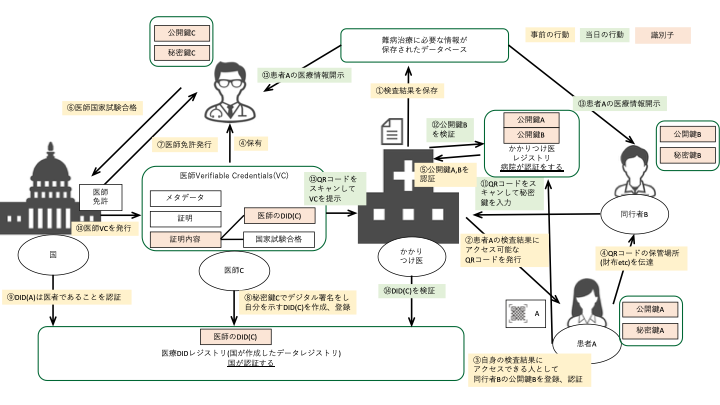
\includegraphics[width=150mm]{VC1.png}}
    \end{center}
    \caption{VC発行までの流れ}
    \label{fig:sample3}
\end{figure}


\subsection{ユースケースに沿ったデータの流れ}

ここでは図\ref{fig:sample1}について、各項目のシステム的な詳細を示す。

\subsubsection{医療情報があるデータベースを作成する}
a.	データベースを作る 
i.	入力テンプレを用意、それを数値別に保存 
ii.	入力画面 
 
 
b.	患者の文書データを保存する。(サーバー)医療サーバー内 
i.	入力元:医師Aのパソコン 
ii.	入力データ:検査結果の数値データ 
iii.	入力先:医療サーバー内のデータベース 
 
 
c.	応急処置と検査結果の見分けがつくようにする。(サーバー)医療サーバー内 
i.	処理:検査結果を示す識別子と応急処置を示す識別子を設定する 
 
 
d.	患者のものと特定できるようにする。(サーバー)医療サーバー内 
i.	処理:保存データに特定の患者を示す識別子を設定する 
 
\subsubsection{患者の医療情報と応急処置情報があるデータベースの位置を示すQRコードを発行する}
a.	位置情報を示すURLの発行。(サーバー) 医療サーバー内 
i.	処理:患者の識別子と検査結果、応急処置の識別子を結びつける 
 
 
b.	QRコードの発行。(サーバー) 医療サーバー内 
i.	処理:URLをQRコードに変換(ライブラリを発動) 
 
\subsubsection{カードの保管場所を知らせる(口頭及びチャットアプリなど)}
 
\subsubsection{QRコードをスキャンする機能を持つデバイス(モバイルアプリetc)でスキャンする}
a.	URLの情報を得る。ライブラリを使う(モバイルアプリ)QRコードからモバイル端末にURL情報の伝達 
i.	問い合わせ元:モバイルアプリ 
ii.	処理:モバイルアプリでQRコードを読み、URLに変換 
iii.	問い合わせ先:医療サーバー 
 
\subsubsection{QRコードのアクセス情報に従いデータベースを参照する(図\ref{fig:sample2})}
a.	URLの先でVCの確認画面を表示する。(モバイルアプリ)サーバーからモバイル端末へVCの要求 
i.	出力元:医療サーバー 
ii.	出力:VCの入力画面(HTML) 
iii.	出力先:モバイルアプリ 
 
 
b.	VCの入力があったらそれを病院データベースに送る。(モバイルアプリ)医師のモバイル端末から医療サーバにVCを送る(1 or 2) 
i.	入力元:モバイルアプリ 
ii.	入力データ:医師BのVC 
iii.	入力先:医療サーバー 
 
\subsubsection{医師BのVCの検証}
a.	VC同様の働きをするもの(医師か否かをy/nで判別できる機能があればよく、実際にVCの発行、検証を行うフェーズは7月時点の実装の段階では対象外とする)を検証し、医師か判別する。(サーバー)サーバー内 
i.	入力データ:医師BのVC 
ii.	出力:true/false 
 
\subsubsection{医師Aの公開鍵で署名を複合して検証する(現段階ではここの検証は重視しない)}
 
\subsubsection{なんのデータを送るかを決定する}
a.	VCの提示があった方へ検査結果を送る。(サーバー)サーバーから医師のモバイル端末へ検査結果を表示する 
i.	入力データ:医師BのVC 
ii.	出力:true 
iii.	出力:検査結果の識別子 
iv.	出力データ:検査結果内容 
v.	出力先:医師Bのモバイルアプリ 
 
 
b.	そうでない方には応急処置を送る。(サーバー)サーバーから同行者のモバイル端末へ応急処置情報を表示する。 
i.	入力データ:N/A or 間違ったVC 
ii.	出力:false 
iii.	出力:応急処置の識別子 
iv.	出力データ:応急処置内容 
v.	出力先:同行者のモバイルアプリ 
 
\subsubsection{それぞれの端末に表示する。}
a.	必要な情報のデータを表示する。(サーバー)サーバーからそれぞれの端末に情報を表示 
i.	出力データ:検査結果/応急処置 
ii.	処理:web上にHTMLで一時的に患者の医療情報のページを作成 
iii.	出力先:web 
 
 
b.	端末側で表示させる。(モバイルアプリ)モバイル端末内 
i.	出力元:医療サーバー 
ii.	出力データ:webページの位置 
iii.	出力先:モバイルアプリ 



\begin{figure}[htbp]
    \begin{center}
       \fbox{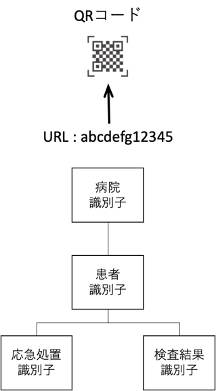
\includegraphics[width=50mm]{ID.png}}
    \end{center}
    \caption{QRコードから取得する患者の情報}
    \label{fig:sample2}
\end{figure}


\section{結果}
\subsection{従来方式との項目別評価}
\subsection{従来方式とのフロー比較}




\begin{comment}
\section{まとめ}

\LaTeX の環境さえあればスタンダードな体裁の論文がたぶんだれでも作れる程度のテンプレートにはなっているはず。がんばって卒業しよう。


\section{大事なこと}

箇条書きで列挙する。

\begin{itemize}
 \item ぐぐる。これは単なる\LaTeX だし、\LaTeX はもう枯れた技術だから、調べれば文献はいくらでもある。
 \item 先生を頼る。
 \item 単位をきちんとる。
 \item 卒業する。
\end{itemize}

\end{comment}